% Options for packages loaded elsewhere
\PassOptionsToPackage{unicode}{hyperref}
\PassOptionsToPackage{hyphens}{url}
\PassOptionsToPackage{dvipsnames,svgnames*,x11names*}{xcolor}
%
\documentclass[
  11pt,
]{article}
\usepackage[]{mathpazo}
\usepackage{amsmath}
\usepackage{ifxetex,ifluatex}
\ifnum 0\ifxetex 1\fi\ifluatex 1\fi=0 % if pdftex
  \usepackage[T1]{fontenc}
  \usepackage[utf8]{inputenc}
  \usepackage{textcomp} % provide euro and other symbols
  \usepackage{amssymb}
\else % if luatex or xetex
  \usepackage{unicode-math}
  \defaultfontfeatures{Scale=MatchLowercase}
  \defaultfontfeatures[\rmfamily]{Ligatures=TeX,Scale=1}
\fi
% Use upquote if available, for straight quotes in verbatim environments
\IfFileExists{upquote.sty}{\usepackage{upquote}}{}
\IfFileExists{microtype.sty}{% use microtype if available
  \usepackage[]{microtype}
  \UseMicrotypeSet[protrusion]{basicmath} % disable protrusion for tt fonts
}{}
\usepackage{xcolor}
\IfFileExists{xurl.sty}{\usepackage{xurl}}{} % add URL line breaks if available
\IfFileExists{bookmark.sty}{\usepackage{bookmark}}{\usepackage{hyperref}}
\hypersetup{
  pdftitle={Making Migration Sexy: Immigrants in Same-Sex Couples in the United States},
  pdfauthor={Nathan I. Hoffmann, Department of Sociology, University of California, Los Angeles; Kristopher Velasco, Department of Sociology, University of Texas at Austin},
  colorlinks=true,
  linkcolor=blue,
  filecolor=Maroon,
  citecolor=Blue,
  urlcolor=Blue,
  pdfcreator={LaTeX via pandoc}}
\urlstyle{same} % disable monospaced font for URLs
\usepackage[margin=1in]{geometry}
\usepackage{longtable,booktabs}
\usepackage{calc} % for calculating minipage widths
% Correct order of tables after \paragraph or \subparagraph
\usepackage{etoolbox}
\makeatletter
\patchcmd\longtable{\par}{\if@noskipsec\mbox{}\fi\par}{}{}
\makeatother
% Allow footnotes in longtable head/foot
\IfFileExists{footnotehyper.sty}{\usepackage{footnotehyper}}{\usepackage{footnote}}
\makesavenoteenv{longtable}
\usepackage{graphicx}
\makeatletter
\def\maxwidth{\ifdim\Gin@nat@width>\linewidth\linewidth\else\Gin@nat@width\fi}
\def\maxheight{\ifdim\Gin@nat@height>\textheight\textheight\else\Gin@nat@height\fi}
\makeatother
% Scale images if necessary, so that they will not overflow the page
% margins by default, and it is still possible to overwrite the defaults
% using explicit options in \includegraphics[width, height, ...]{}
\setkeys{Gin}{width=\maxwidth,height=\maxheight,keepaspectratio}
% Set default figure placement to htbp
\makeatletter
\def\fps@figure{htbp}
\makeatother
\setlength{\emergencystretch}{3em} % prevent overfull lines
\providecommand{\tightlist}{%
  \setlength{\itemsep}{0pt}\setlength{\parskip}{0pt}}
\setcounter{secnumdepth}{-\maxdimen} % remove section numbering
\usepackage{fancyhdr}
\pagestyle{fancy}
\setlength{\headheight}{13.6pt}
\rhead{\textit{Hoffmann and Velasco}}
\ifluatex
  \usepackage{selnolig}  % disable illegal ligatures
\fi
\newlength{\cslhangindent}
\setlength{\cslhangindent}{1.5em}
\newlength{\csllabelwidth}
\setlength{\csllabelwidth}{3em}
\newenvironment{CSLReferences}[2] % #1 hanging-ident, #2 entry spacing
 {% don't indent paragraphs
  \setlength{\parindent}{0pt}
  % turn on hanging indent if param 1 is 1
  \ifodd #1 \everypar{\setlength{\hangindent}{\cslhangindent}}\ignorespaces\fi
  % set entry spacing
  \ifnum #2 > 0
  \setlength{\parskip}{#2\baselineskip}
  \fi
 }%
 {}
\usepackage{calc}
\newcommand{\CSLBlock}[1]{#1\hfill\break}
\newcommand{\CSLLeftMargin}[1]{\parbox[t]{\csllabelwidth}{#1}}
\newcommand{\CSLRightInline}[1]{\parbox[t]{\linewidth - \csllabelwidth}{#1}\break}
\newcommand{\CSLIndent}[1]{\hspace{\cslhangindent}#1}

\title{Making Migration Sexy: Immigrants in Same-Sex Couples in the United States}
\author{Nathan I. Hoffmann, Department of Sociology, University of California, Los Angeles \and Kristopher Velasco, Department of Sociology, University of Texas at Austin}
\date{January 27, 2021}

\begin{document}
\maketitle

\begin{figure}
\centering
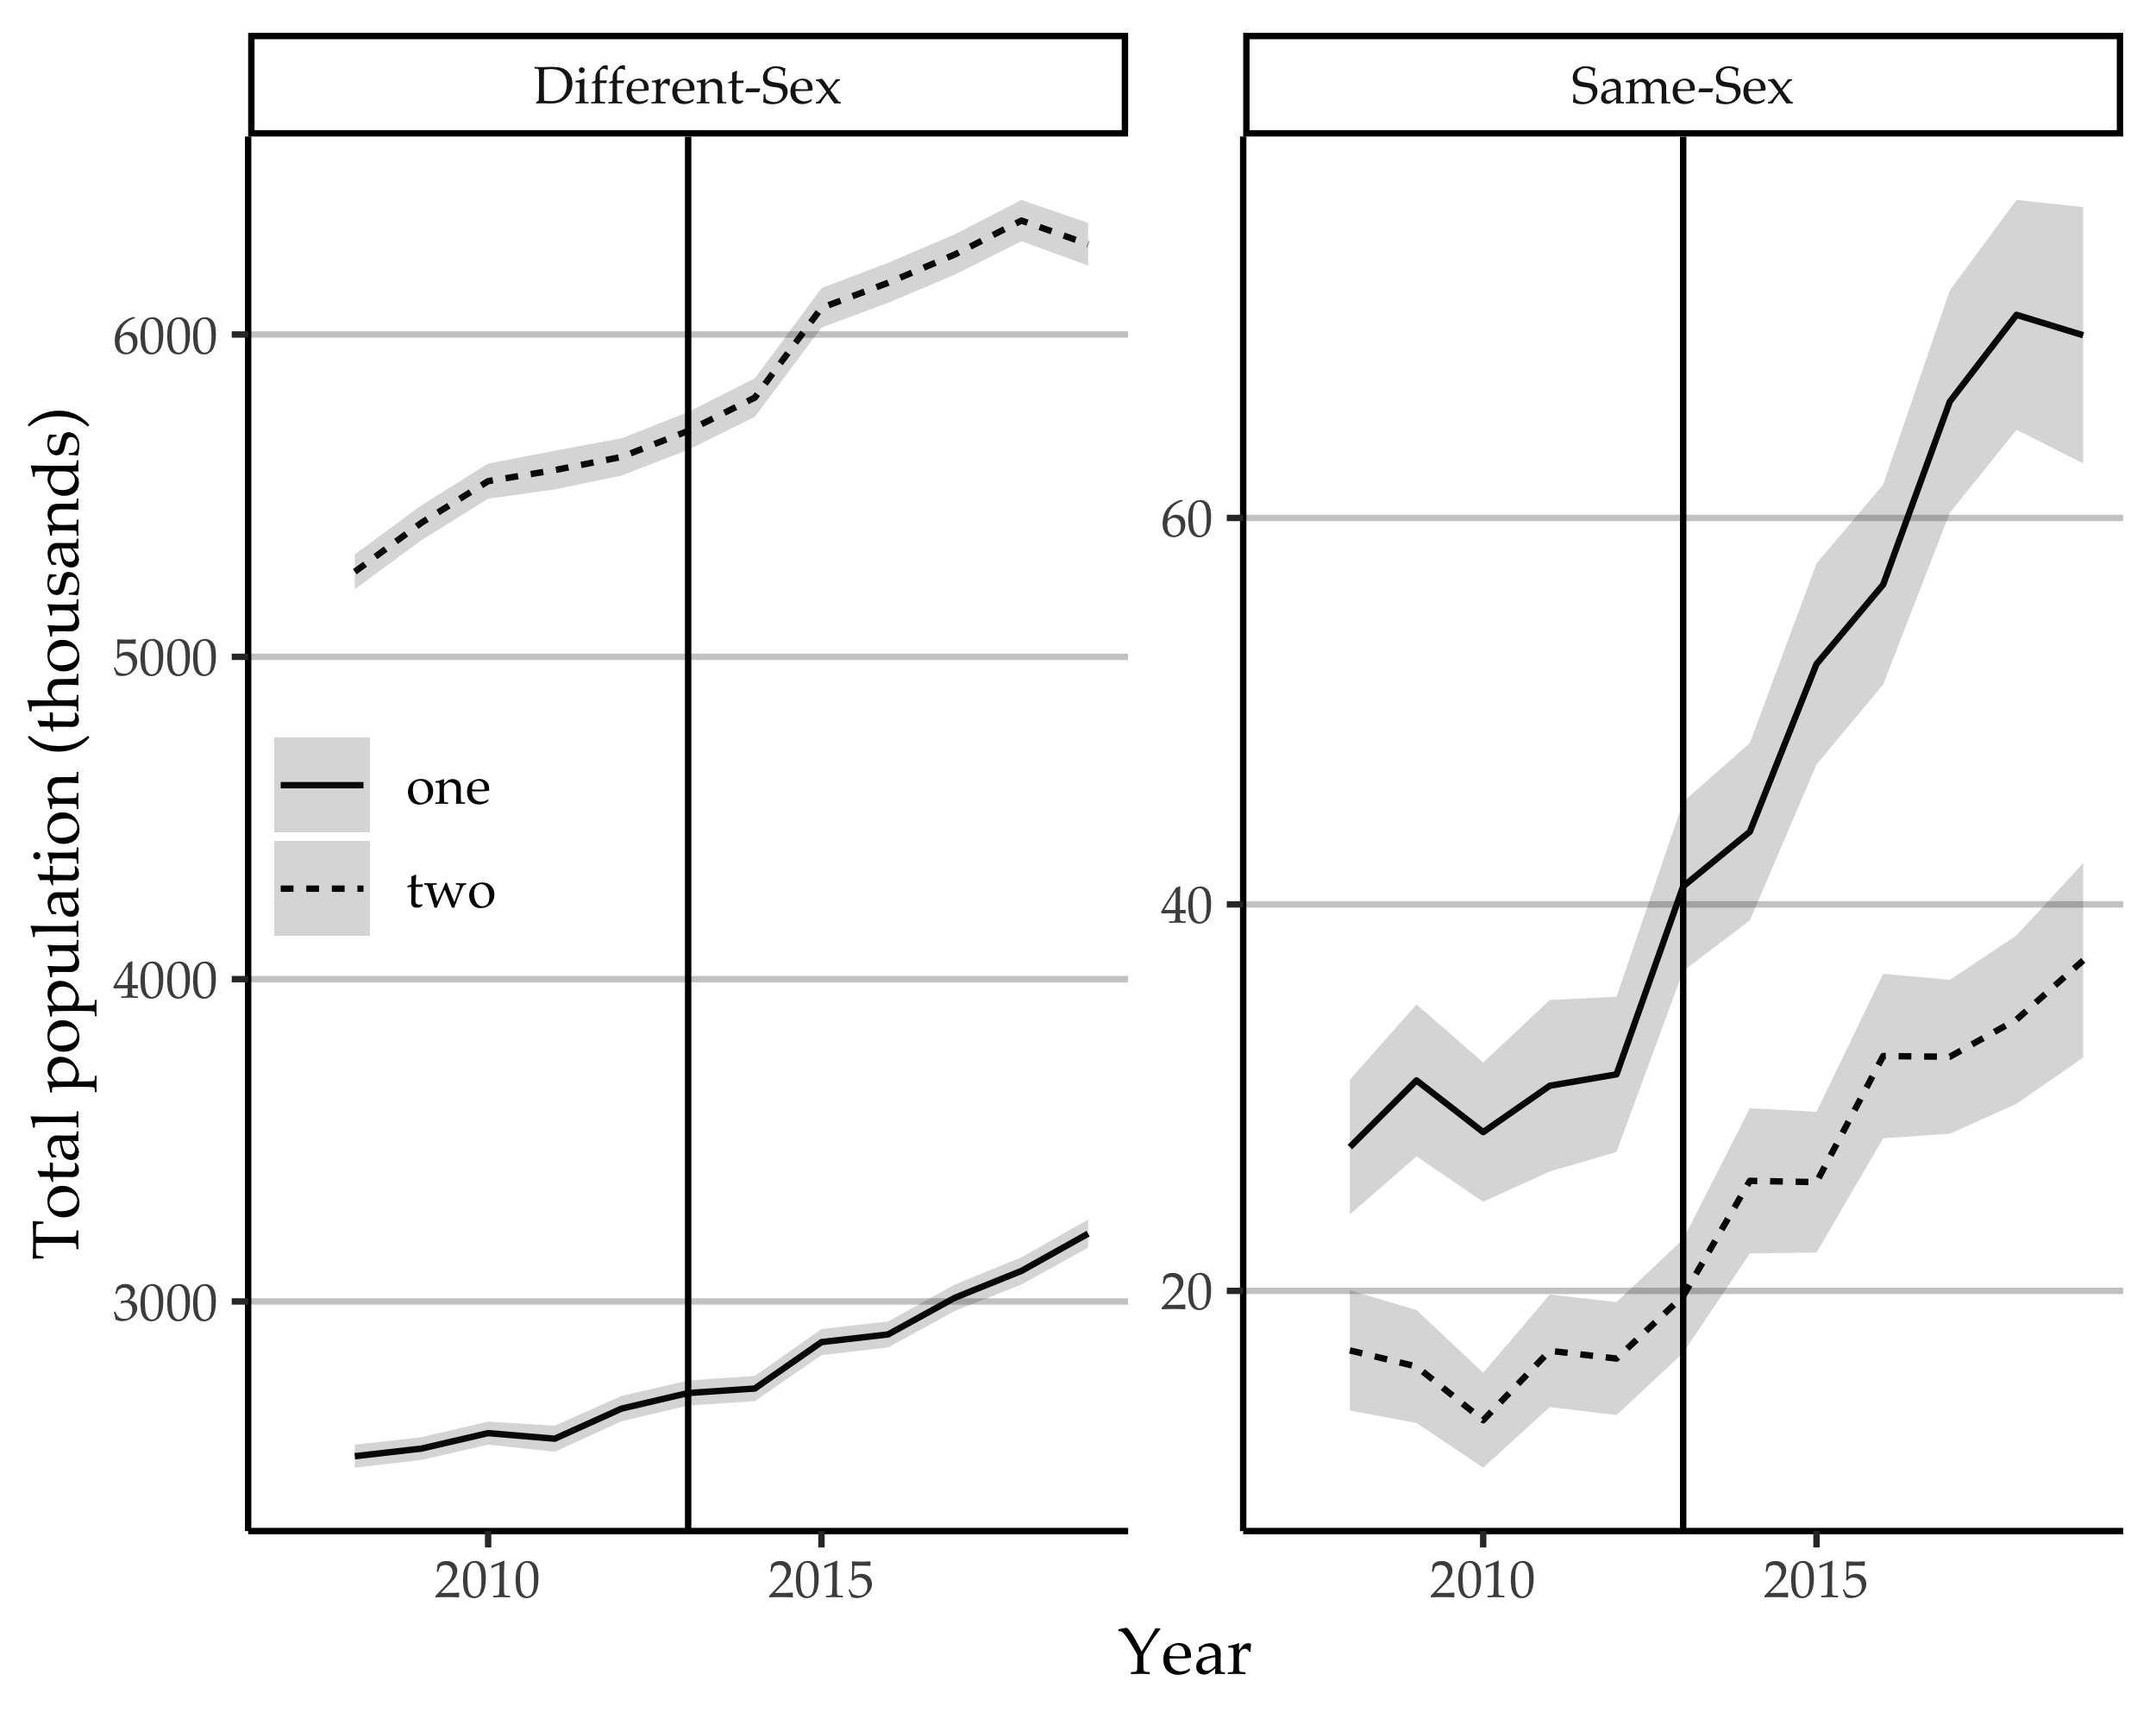
\includegraphics{ssimm_draft_methods_results_files/figure-latex/total-pop-1.pdf}
\caption{\label{fig:total-pop}Estimated totals of different- and same-sex couples containing one or two immigrants, 2008-2019, with 95\% confidence intervals. Vertical line placed at the year 2013, when DOMA was overturned.}
\end{figure}

\hypertarget{understanding-influences-on-migration-patterns}{%
\section{Understanding Influences on Migration Patterns}\label{understanding-influences-on-migration-patterns}}

\hypertarget{conventional-explanations}{%
\subsection{Conventional Explanations}\label{conventional-explanations}}

Dominant theories in migration fail to explain the rapid rise of immigrants in same-sex couples in the U.S. For at least two decades, migration scholars have accepted the conclusion of Massey et al. (\protect\hyperlink{ref-massey_1999}{1999, 50}) that ``causal processes relevant to international migration might operate on multiple levels simultaneously.'' Whereas economic theories underscore that promise of material gain is a frequent motivation to migrate (\protect\hyperlink{ref-hatton_2005a}{Hatton and Williamson 2005}), structural explanations point to how the disruption of local economies by global forces spurs out-migration (\protect\hyperlink{ref-piore_1979}{Piore 1979}; \protect\hyperlink{ref-wallerstein_1979}{Wallerstein 1979}). Network theory explains for why migration streams often continue to flow in full force even after wage differentials decrease (\protect\hyperlink{ref-massey_1987}{Massey et al. 1987}), while work on the ``migration industry'' shows how brokers, recruiters, smugglers, and other ``entrepreneurs'' initiate and maintain migrant flows (\protect\hyperlink{ref-hernandez-leon_2013}{Hernández-León 2013}). However, there is little reason to believe that the economic, structural, network, and institutional forces that shape migration of heterosexual immigrants differ from those that affect LGB immigrants. Although these theories do much to help understand broad patterns of migration, they falter in explaining increasing rates of LGB migration.

The problem lies in two conspicuous absences in mainstream migration theory. The first is the lack of a large role for the state. Outside of violent contexts triggering refugee flows (\protect\hyperlink{ref-fitzgerald_2018}{FitzGerald and Arar 2018}), scholars of migration rarely focus on the political factors that both constrain and enable migration in sending and receiving countries. In recent years, some research has emerged that does consider political variables explicitly. For example, on the receiving country side, \protect\hyperlink{ref-fitzgerald_2014}{Fitzgerald, Leblang, and Teets} (\protect\hyperlink{ref-fitzgerald_2014}{2014}) show that safeguards for immigrant rights are important predictors of immigration, even in models that control for the usual ``gravity model'' economic, distance, and network variables. Other scholars have looked at sending-country policies relevant to emigration, such as dual citizenship laws (\protect\hyperlink{ref-leblang_2017}{Leblang 2017}) and autocratic restraints on exit (\protect\hyperlink{ref-miller_2018}{Miller and Peters 2018}). State policy relevant to particular subgroups or not obviously related to migration, however, has received little study.

Second, the dominant migration literature fails to consider how identity might shape migration desires. Recent research in ``lifestyle migration'' (\protect\hyperlink{ref-benson_2012}{Benson and O'Reilly 2012}) begins to probe the non-economic hopes and aspirations that might encourage settling in a new country. And although gender is slowly being recognized as an integral consideration in studies of migration (\protect\hyperlink{ref-lutz_2010}{Lutz 2010}; \protect\hyperlink{ref-hondagneu-sotelo_2012}{Hondagneu-Sotelo 2012}), sexuality has received comparably little attention. Moving beyond the dominant migration theories synthesized by Massey et al. (\protect\hyperlink{ref-massey_1999}{1999}), this paper sheds light on how the intersection of state policy and sexuality shapes migration decisions.

\hypertarget{data}{%
\section{Data}\label{data}}

We merge individual-level data on immigrants in the U.S. with state- and country-level variables from a variety of datasets. The individual data come from the 2008 to 2019 American Community Survey (ACS). Each year, the ACS surveys a 1\% sample of the U.S. population about their education, occupation, income, family structure, immigration status, country of origin, location, and a variety of other individual and household attributes. Although the ACS began in 2000, variables on same-sex partners were not reliable until 2008 (\protect\hyperlink{ref-u.s.censusbureau_2013}{U.S. Census Bureau 2013}). We limit the sample to individuals who immigrated at the age of 18 or older. The 11 years of survey data contain 9,325 same-sex couples that include at least one immigrant, for a total of 12,443 immigrants in same-sex couples. These immigrants are compared to 985,884 corresponding different-sex couples (containing 1,626,731 individual immigrants).

Our explanatory variables of interest are the LGBT policy context in country of origin and U.S. state of residence. To create the U.S. state policy index, we compile data from the Movement Advancement Project, a leading LGBT organization in the U.S. that collects data on a number of relevant policies. Our state index encompasses both progressive policies (full marriage equality, state recognition of civil unions and domestic partnerships, ban on all employment and housing discrimination based on sexual orientation, hate crime protections based on sexual orientation, legal joint adoption by same-sex couples, and a ban on conversation therapy for minors) and regressive policies (criminalization of sodomy, state constitutional bans of marriage equality, religious freedom exemptions to discriminate against same-sex couples in adoption, and state-level bans on local non-discrimination ordinances encompassing sexual orientation). The state index ranges from -2 to 7, and the mean score of country of origin for immigrant in our sample is 3.2.

We measure the origin country policy environment using the LGBT Policy Index (\protect\hyperlink{ref-velasco_2018}{Velasco 2018}). This index comprises 14 policies, many similar to those above, but including additional policies like the death penalty for homosexual acts, propaganda laws limiting free speech for LGBT communities, and equal age of consent between same-sex and opposite-sex couples. Both indices are created by summing the net total of progressive policies (scored \(+1\)) over regressive policies (scored \(-1\)). The state index ranges from -3.2 to 11, and the mean score of country of origin for immigrant in our sample is 1.7.

Immigrants are assigned state index scores (destination policy environment) based on their self-reported state of residence during the year of the ACS survey. They are assigned country index scores (origin policy environment) based on their year of immigration. Since the country policy index begins at 1991, we anyone who immigrated before 1991 gets assigned the 1991 value.

Our country- and state-level controls come from a variety of sources. Country-of-origin controls for bilateral distance, contiguous border, common official language, common ethnic language, and whether the country was a former colony of the U.S. come from CEPII's GeoDist dataset. Difference in wages (in 1000s of 2011 US dollars) come from the Penn World Table, and we rely on World Bank data for differences in unemployment rates. We use Polity5 measures of democratization of the country of origin. For state controls, we use per capita income by year from the Bureau of Economic Analysis and state-level annual unemployment rates from the Bureau of Labor Statistics.

For our individual-level analysis we include individual controls from the ACS for reported sex, age, education (with categories for less than high school, high school, some college, and college), log positive income, and a binary indicator for income reported to be 0 or less.

\hypertarget{analytic-strategy}{%
\section{Analytic Strategy}\label{analytic-strategy}}

Our first goal is to isolate the effects of country-of-origin LGBT policy on the immigration of immigrants in same-sex couples. The ideal survey would follow potential immigrants over time and have information about sexual orientation, allowing us to estimate how the probability of migrating and choice of U.S. state of residence vary by sexual orientation. This ideal dataset does not exist, but we approximate it at the macro level. We take the number of immigrants in same-sex couples from a given country and a given year of immigration and divide by the total number of immigrants from that country-year. If sending-country LGBT policy has no effect on migration rates of LGB immigrants, then we would expect these proportions to be similar between countries. However, LGBT policy may covary with potential confounders such as country income, unemployment, democratization, and relationship to the U.S., so we control for these variables in our preferred model and estimate using ordinary least squares (OLS) regression. We also specify models with country fixed or random effects to account for unobserved heterogeneity within countries. All of these models also have country-clustered standard errors.

Our next set of models focus on U.S. state LGBT policy. We reshape the data so that each observation is the proportion of immigrants in same-sex couples from country \(x\) in state \(y\) in year \(z\). We regress this proportion on state and sending-country policy scores, controlling for the same country- and state-level attributes as in the previous set of models. We include state and country-of-origin fixed effects, and cluster errors at the state level.

Our final set of models turns toward the individual: conditional on immigrating to the U.S., do immigrant in same-sex couples choose more LGBT-friendly states to reside in? This part of the analysis uses ordered logistic regression to predict the policy index of state of residence. Whereas the full U.S. state policy index ranges from -2 to 7, we break up the index into three ``bins'': repressive (0 and less), neutral (1 or 2), and progressive (3 and greater). We control for individual attributes that could possibly confound our results and include survey-year fixed effects and country-clustered standard errors.

\hypertarget{results}{%
\section{Results}\label{results}}

\hypertarget{descriptive-statistics}{%
\subsection{Descriptive statistics}\label{descriptive-statistics}}

We first estimate total numbers of immigrants in same- and different-sex couples, applying survey weights to obtain population-level estimates from the ACS. Figure \ref{fig:total-pop} shows that whereas numbers of different-sex immigrant couples have steadily increased over the period of study, numbers of same-sex immigrant couples have increased much more rapidly, especially since the the 2013 Supreme Court decision overturning DOMA.

Figure \ref{fig:policy-desc} charts the average country-of-origin and U.S.-state policy score for the immigrants in our sample over time, comparing means for immigrants in same- and different-sex couples. The left panel shows that country-of-origin index at time of migration is generally higher for immigrants in same-sex couples, especially in recent years. Immigrants in same-sex couples tend to come from more progressive countries. The left panel indicates less of a difference in U.S. state policies, although states where immigrants in same-sex couples live tend to score somewhat higher.

\begin{figure}
\centering
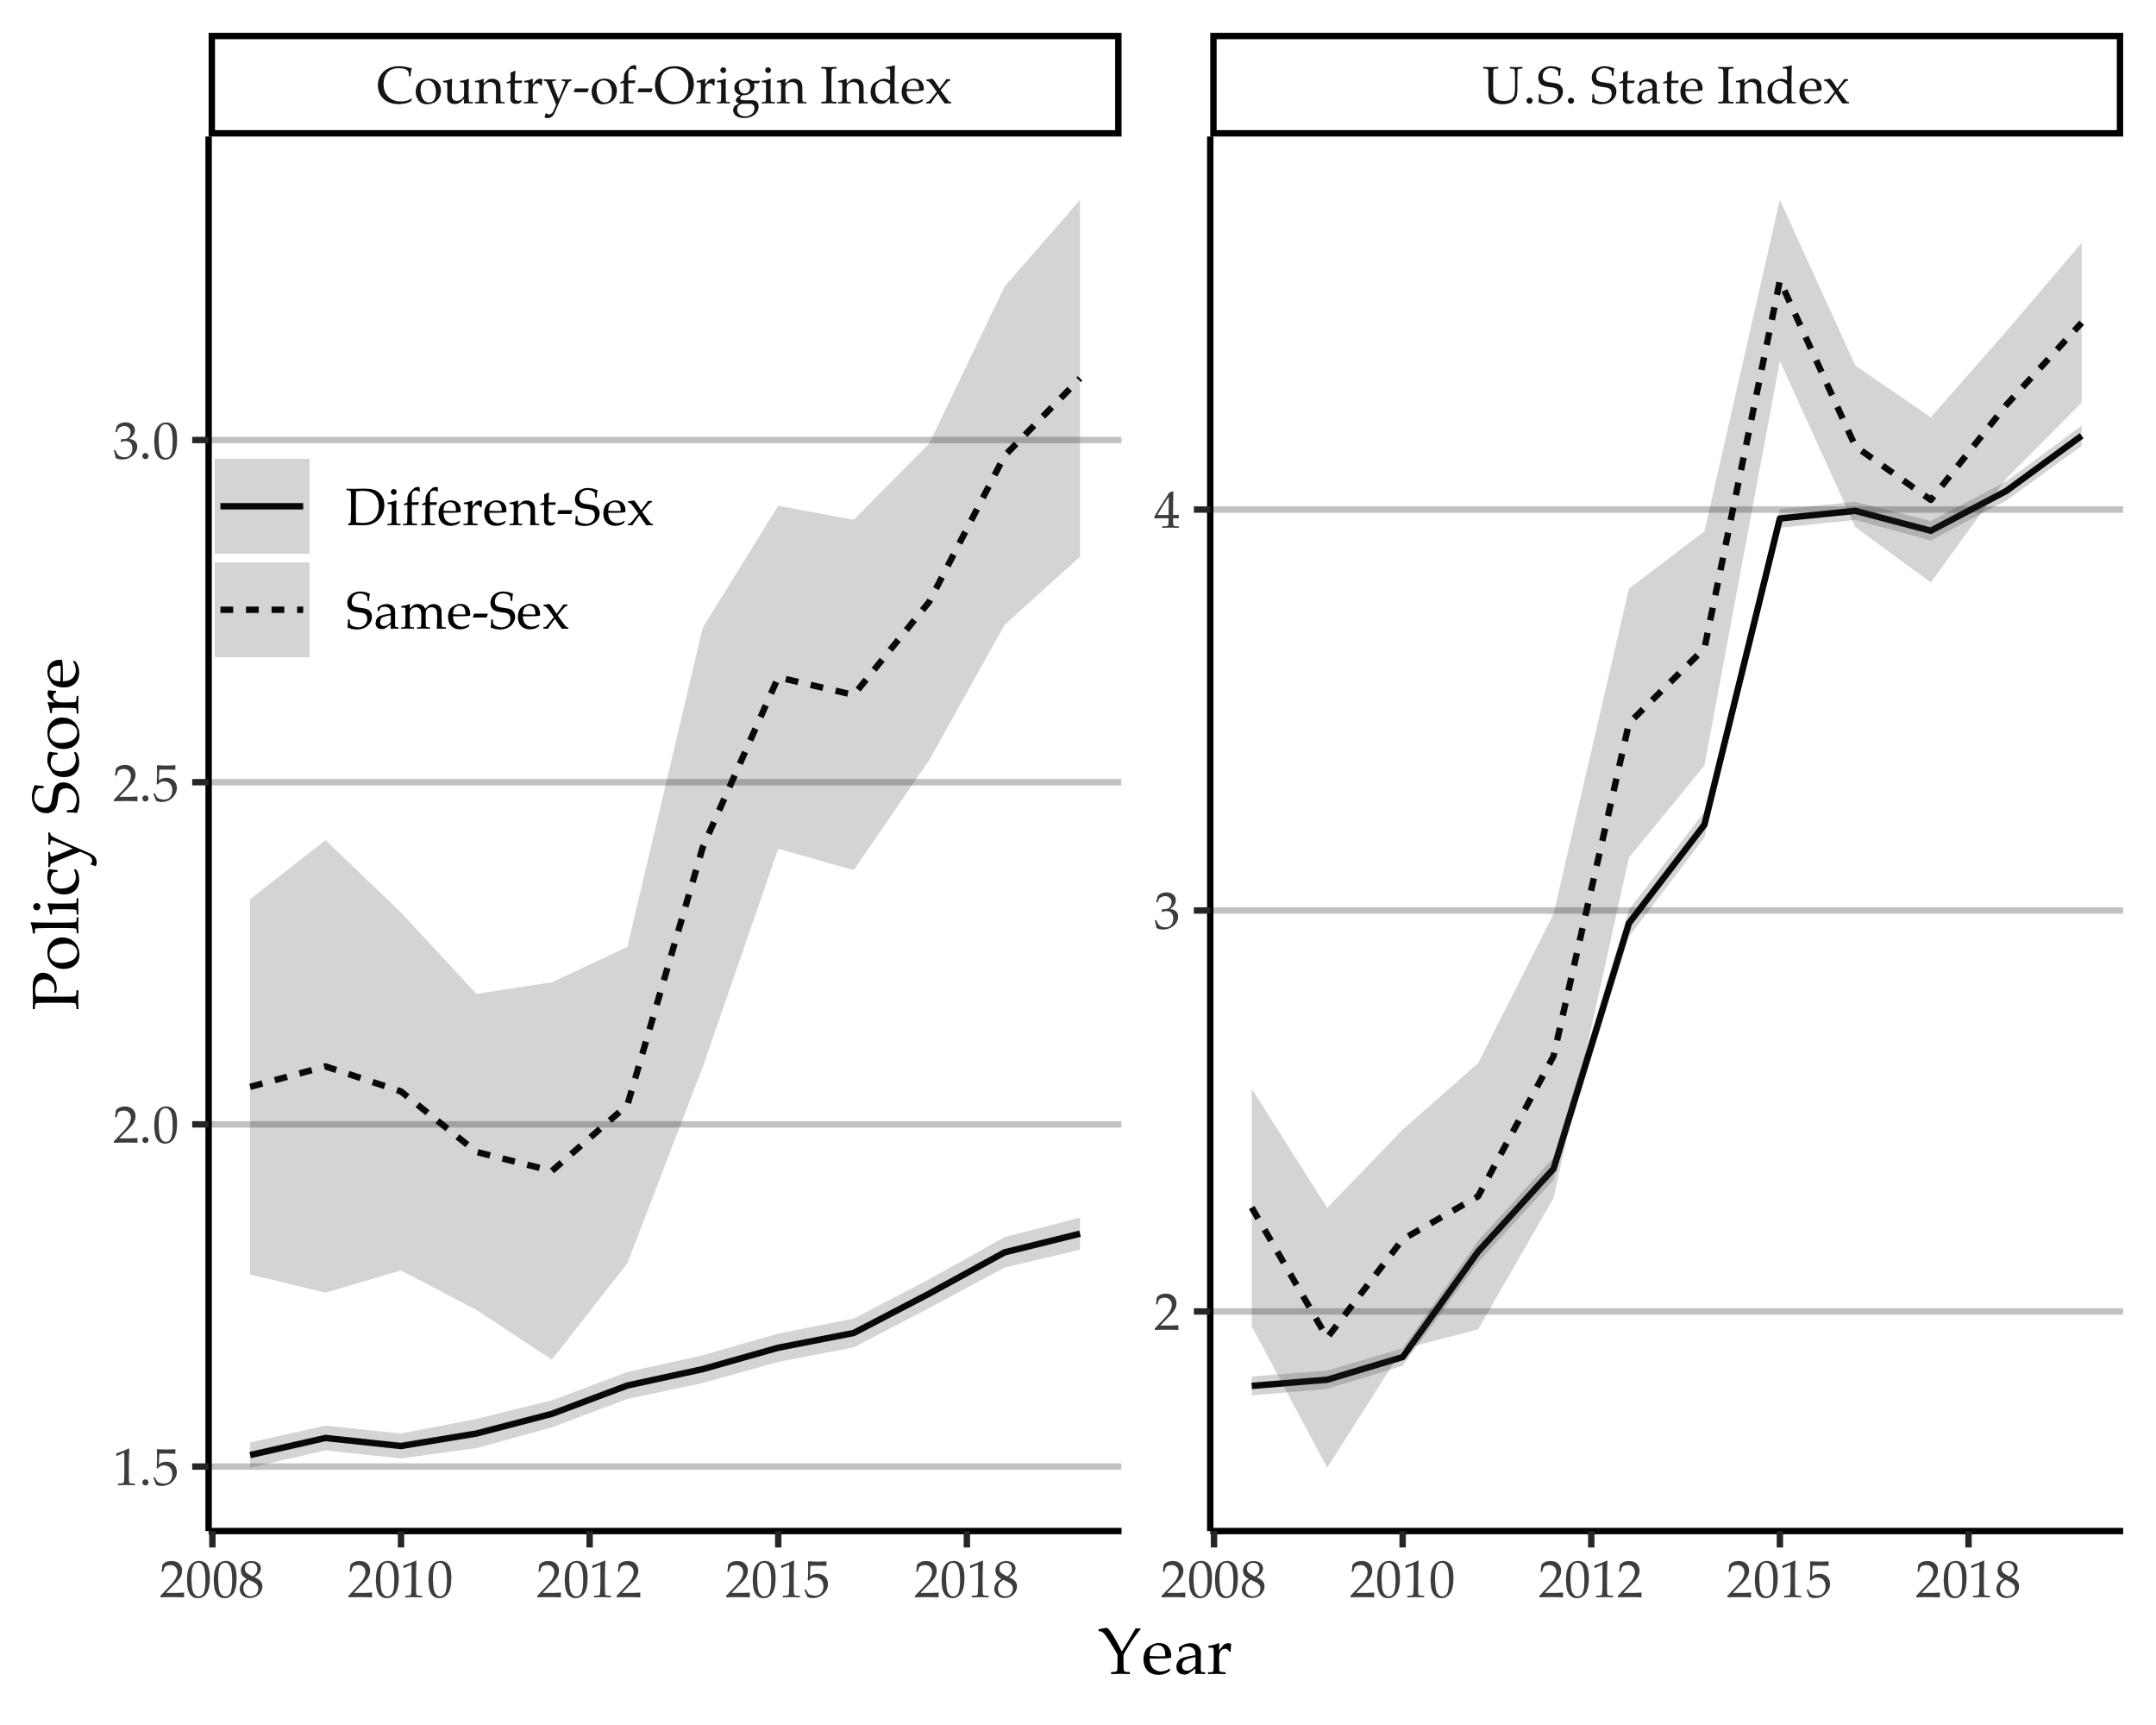
\includegraphics{ssimm_draft_methods_results_files/figure-latex/policy-desc-1.pdf}
\caption{\label{fig:policy-desc}Mean country-of-origin and U.S. state policy index score for immigrants in same- and different-sex couples, 2008-2019, with 95\% confidence intervals.}
\end{figure}

\begin{table}

\caption{\label{tab:country-tab}Sending countries ranked bby proportion immigrant couples with same-sex partners}
\centering
\begin{tabular}[t]{lllr}
\toprule
Rank & Country of origin & Proportion same-sex & Mean policy score\\
\midrule
1 & Australia & 2.53 \% & 4.08\\
2 & Mongolia & 2.37 \% & 2.25\\
3 & Belgium & 2.25 \% & 4.98\\
4 & New Zealand & 2.12 \% & 5.43\\
5 & Singapore & 2.11 \% & -0.20\\
6 & Netherlands & 2.08 \% & 7.15\\
7 & France & 2.05 \% & 6.07\\
8 & Malaysia & 2.05 \% & -0.89\\
9 & Zimbabwe & 2.01 \% & -0.95\\
10 & Spain & 1.98 \% & 5.60\\
\bottomrule
\end{tabular}
\end{table}

\begin{table}

\caption{\label{tab:state-tab}States ranked by proportion immigrant couples with same-sex partners}
\centering
\begin{tabular}[t]{lllr}
\toprule
Rank & State & Proportion same-sex & Mean policy score\\
\midrule
1 & Vermont & 2.09 \% & 5.17\\
2 & Maine & 1.63 \% & 4.79\\
3 & Montana & 1.47 \% & 0.81\\
4 & Missouri & 1.18 \% & 1.91\\
5 & Massachusetts & 1.12 \% & 4.77\\
6 & New York & 1.10 \% & 4.84\\
7 & Florida & 1.01 \% & 0.91\\
8 & Mississippi & 1.00 \% & -0.49\\
9 & Minnesota & 0.96 \% & 4.63\\
10 & New Hampshire & 0.95 \% & 4.33\\
\bottomrule
\end{tabular}
\end{table}

Table \ref{tab:country-tab} ranks the proportion of U.S. immigrants in same-sex couples based on country of origin, averaging over the 11 years of survey data. The top sending countries mostly hold more progressive policies, but Singapore, Malaysia, and Zimbabwe maintain generally repressive policies at the year of departure of the immigrants in our sample. Table \ref{tab:state-tab} similarly ranks U.S. state by the proportion of immigrants in same-sex couples, averaging over the period of interest. Although states with progressive policies make the top of the list, Mississippi is somewhat repressive, and Montana, Missouri, and Florida hold more neutral policies.

\hypertarget{models}{%
\subsection{Models}\label{models}}

\begin{table}[!htbp] \centering 
  \caption{Percent of immigrants in same-sex couples by year of immigration and country of origin.} 
  \label{tab:country-props} 
\begin{tabular}{@{\extracolsep{5pt}}lcccc} 
\\[-1.8ex]\hline 
\hline \\[-1.8ex] 
 & \multicolumn{4}{c}{\textit{Dependent variable:}} \\ 
\cline{2-5} 
\\[-1.8ex] & \multicolumn{4}{c}{prop\_same\_sex} \\ 
\\[-1.8ex] & (1) & (2) & (3) & (4)\\ 
\hline \\[-1.8ex] 
 distw &  & 0.00003$^{**}$ & 0.002$^{*}$ & 0.00003$^{+}$ \\ 
  &  & (0.00001) & (0.001) & (0.00001) \\ 
  & & & & \\ 
 contig &  & $-$0.037 & 2.500$^{+}$ & $-$0.039 \\ 
  &  & (0.200) & (1.500) & (0.290) \\ 
  & & & & \\ 
 comlang\_off &  & 0.003 & $-$17.000$^{*}$ & 0.006 \\ 
  &  & (0.081) & (7.900) & (0.120) \\ 
  & & & & \\ 
 comlang\_ethno &  & 0.010 & 8.500$^{*}$ & 0.001 \\ 
  &  & (0.069) & (3.800) & (0.100) \\ 
  & & & & \\ 
 colony &  & 0.120 & 12.000$^{*}$ & 0.150 \\ 
  &  & (0.140) & (5.700) & (0.200) \\ 
  & & & & \\ 
 wage\_dif &  & $-$0.00001 & 0.00001 & $-$0.00000 \\ 
  &  & (0.00001) & (0.00001) & (0.00001) \\ 
  & & & & \\ 
 unemp\_dif &  & $-$0.002 & 0.005 & $-$0.0005 \\ 
  &  & (0.004) & (0.009) & (0.005) \\ 
  & & & & \\ 
 polity5 &  & 0.023$^{***}$ & 0.0004 & 0.020$^{***}$ \\ 
  &  & (0.005) & (0.010) & (0.006) \\ 
  & & & & \\ 
 origin\_score & 0.079$^{***}$ & 0.066$^{***}$ & 0.037$^{+}$ & 0.062$^{***}$ \\ 
  & (0.007) & (0.010) & (0.019) & (0.013) \\ 
  & & & & \\ 
\hline \\[-1.8ex] 
Country-clustered SEs? & yes & yes & yes & NA \\ 
Country FEs? & no & no & yes & no \\ 
Country REs? & no & no & no & yes \\ 
Observations & 3,811 & 2,995 & 2,995 & 2,995 \\ 
R$^{2}$ & 0.031 & 0.041 & 0.120 &  \\ 
\hline 
\hline \\[-1.8ex] 
\textit{Note:}  & \multicolumn{4}{r}{+p<0.1; *p<0.05; **p<0.01; ***p<0.001} \\ 
\end{tabular} 
\end{table}

Our first set of models predicts the percent of immigrants in same-sex couples by country of origin and year of immigration (Table \ref{tab:country-props}). Model 1 regresses this proportion on only our variable of interest: LGBT policy score in country of origin. We see that countries with more progressive LGBT policy tend to send more immigrants to the U.S. who end up in same-sex couples. The average proportion of immigrants in same-sex couples is only \texttt{r}mean(acs\_prop\_yrimmig\_policy\$prop\_same\_sex, na.rm = T)` percent, so an increase of 0.079 per point increase in LGBT policy score represents a substantive effect.

The other models in Table \ref{tab:country-props} assess the robustness of this finding. Model 2 includes typical controls from gravity models of immigration (e.g. \protect\hyperlink{ref-fitzgerald_2014}{Fitzgerald, Leblang, and Teets 2014}) along with a measure of democratization. The coefficient for country-of-origin score reduces slightly but remains highly significant. Notably, it is estimated to be three times the effect size of democratization score; the LGBT policy environment matters much more than the overall progressiveness of government policy. Models 3 and 4 include country-of-origin fixed and random effects, respectively. Although in the fixed effects model coefficient for origin score is reduced by half compared to Model 1, it remains significant at the \(\alpha = 0.1\) level. The corresponding coefficient random effects model remains large and statistically significant.

\begin{table}[!htbp] \centering 
  \caption{Percent same-sex in by country of origin, U.S. state, and survey year.} 
  \label{tab:state-props} 
\begin{tabular}{@{\extracolsep{5pt}}lccc} 
\\[-1.8ex]\hline 
\hline \\[-1.8ex] 
 & \multicolumn{3}{c}{\textit{Dependent variable:}} \\ 
\cline{2-4} 
\\[-1.8ex] & \multicolumn{3}{c}{same\_prop} \\ 
\\[-1.8ex] & (1) & (2) & (3)\\ 
\hline \\[-1.8ex] 
 state\_unemploy &  & $-$0.033$^{+}$ & $-$0.001 \\ 
  &  & (0.017) & (0.023) \\ 
  & & & \\ 
 state\_income &  & 0.00001 & $-$0.00003 \\ 
  &  & (0.00001) & (0.00002) \\ 
  & & & \\ 
 origin\_score & 0.053$^{***}$ & 0.050$^{***}$ & 0.110$^{**}$ \\ 
  & (0.011) & (0.011) & (0.040) \\ 
  & & & \\ 
 distw &  &  & 0.004$^{***}$ \\ 
  &  &  & (0.001) \\ 
  & & & \\ 
 contig &  &  & 5.900$^{***}$ \\ 
  &  &  & (1.600) \\ 
  & & & \\ 
 comlang\_off &  &  & $-$35.000$^{***}$ \\ 
  &  &  & (8.600) \\ 
  & & & \\ 
 comlang\_ethno &  &  & 18.000$^{***}$ \\ 
  &  &  & (4.100) \\ 
  & & & \\ 
 colony &  &  & 26.000$^{***}$ \\ 
  &  &  & (6.200) \\ 
  & & & \\ 
 wage\_dif &  &  & 0.0001$^{**}$ \\ 
  &  &  & (0.0001) \\ 
  & & & \\ 
 unemp\_dif &  &  & $-$0.022$^{+}$ \\ 
  &  &  & (0.012) \\ 
  & & & \\ 
 polity5 &  &  & $-$0.001 \\ 
  &  &  & (0.012) \\ 
  & & & \\ 
 state\_policy & 0.033$^{+}$ & 0.008 & 0.041 \\ 
  & (0.017) & (0.034) & (0.036) \\ 
  & & & \\ 
\hline \\[-1.8ex] 
State-clustered SEs? & yes & yes & yes \\ 
State FEs? & no & yes & yes \\ 
Country FEs? & no & no & yes \\ 
Observations & 44,431 & 44,076 & 39,147 \\ 
R$^{2}$ & 0.001 & 0.003 & 0.010 \\ 
\hline 
\hline \\[-1.8ex] 
\textit{Note:}  & \multicolumn{3}{r}{+p<0.1; *p<0.05; **p<0.01; ***p<0.001} \\ 
\end{tabular} 
\end{table}

Table \ref{tab:state-props} presents models of U.S. state-level proportion of immigrants in same-sex couples, from a given country of origin in a given survey year. Model 1 contains only two predictors: U.S. state policy score in the survey year and country-of-origin policy score at the mean year of immigration. Although more LGBT-friendly policies in both locations are associated with higher numbers of immigrants in same-sex couples, country-of-origin LGBT policy is a stronger predictor than U.S. state policy, even considering the somewhat different scale of these variables. A one-standard deviation increase origin score is associated with a 0.11 percentage-point increase of immigrants in same-sex couples, whereas the corresponding state policy effect is 0.079 percentage points.

Model 2 adds state-level controls and fixed effects. Immigrants in same-sex couples may be attracted to progressive states for their economic rather than political benefits. Indeed, in this model, the coefficient for state policy is reduced and rendered insignificant. Model 3 adds country-of-origin controls and fixed effects. The state policy effect remains imprecisely estimated, but country-of-origin policy has increased in strength. More progressive sending countries are more represented among same-sex couples, while U.S. state policy appears to have little influence on their settlement patterns, at least in the aggregate.

\begin{table}[!htbp] \centering 
  \caption{Individual ordered logit analysis of three-category state policy score} 
  \label{tab:ord} 
\begin{tabular}{@{\extracolsep{5pt}}lccc} 
\\[-1.8ex]\hline 
\hline \\[-1.8ex] 
 & \multicolumn{3}{c}{\textit{Dependent variable:}} \\ 
\cline{2-4} 
\\[-1.8ex] & \multicolumn{3}{c}{state\_policy\_binned} \\ 
\\[-1.8ex] & (1) & (2) & (3)\\ 
\hline \\[-1.8ex] 
 same\_sex & 0.160$^{***}$ & 0.100$^{***}$ & 20.000$^{***}$ \\ 
  & (0.020) & (0.027) & (0.0003) \\ 
  origin\_score &  & $-$0.051$^{***}$ & $-$0.022$^{***}$ \\ 
  &  & (0.003) & (0.003) \\ 
  sexMale &  &  & $-$0.059$^{***}$ \\ 
  &  &  & (0.013) \\ 
  age &  &  & 0.001$^{+}$ \\ 
  &  &  & (0.001) \\ 
  educcollege &  &  & 0.070$^{***}$ \\ 
  &  &  & (0.010) \\ 
  educHS &  &  & $-$0.036$^{***}$ \\ 
  &  &  & (0.011) \\ 
  educsome col &  &  & $-$0.023$^{*}$ \\ 
  &  &  & (0.011) \\ 
  nchild &  &  & 0.045$^{***}$ \\ 
  &  &  & (0.006) \\ 
  log\_income &  &  & 0.070$^{***}$ \\ 
  &  &  & (0.002) \\ 
  no\_income &  &  & 0.610$^{***}$ \\ 
  &  &  & (0.002) \\ 
  yrimmig &  &  & $-$0.020$^{***}$ \\ 
  &  &  & (0.00002) \\ 
  same\_sexTRUE:origin\_score &  & 0.038$^{***}$ & 0.052$^{***}$ \\ 
  &  & (0.008) & (0.009) \\ 
  same\_sexTRUE:sexMale &  &  & 0.041$^{***}$ \\ 
  &  &  & (0.002) \\ 
  same\_sexTRUE:age &  &  & $-$0.005$^{***}$ \\ 
  &  &  & (0.002) \\ 
  same\_sexTRUE:educcollege &  &  & 0.120$^{***}$ \\ 
  &  &  & (0.003) \\ 
  same\_sexTRUE:educHS &  &  & 0.005$^{**}$ \\ 
  &  &  & (0.002) \\ 
  same\_sexTRUE:educsome col &  &  & 0.064$^{***}$ \\ 
  &  &  & (0.001) \\ 
  same\_sexTRUE:nchild &  &  & $-$0.017 \\ 
  &  &  & (0.021) \\ 
  same\_sexTRUE:log\_income &  &  & 0.029$^{***}$ \\ 
  &  &  & (0.006) \\ 
  same\_sexTRUE:no\_income &  &  & 0.290$^{***}$ \\ 
  &  &  & (0.001) \\ 
  same\_sexTRUE:yrimmig &  &  & $-$0.010$^{***}$ \\ 
  &  &  & (0.0001) \\ 
 \hline \\[-1.8ex] 
Country-clustered SEs? & yes & yes & yes \\ 
Survey year FEs? & yes & yes & yes \\ 
Observations & 111,880 & 107,168 & 107,168 \\ 
\hline 
\hline \\[-1.8ex] 
\textit{Note:}  & \multicolumn{3}{r}{+p<0.1; *p<0.05; **p<0.01; ***p<0.001} \\ 
\end{tabular} 
\end{table}

Our final set of models turn to the individual. Conditional on migrating to the U.S., do immigrants in same-sex couples choose to live in more progressive states than their heterosexual counterparts? Table \ref{tab:ord} presents ordered logit models predicting whether an individual partnered immigrant lives in a U.S. state with repressive, neutral, or progressive LGBT policies, pooling data across survey years. Model 1 includes only one regressor: an indicator for whether the immigrant is in a same-sex couple. The positive coefficient indicates that immigrants in same-sex couples indeed tend to live in states with more LGBT-friendly policies. The predicted probability for an immigrant in a different-sex couple to live in a state with progressive LGBT policies is 0.6, whereas the corresponding probability for those in same-sex couples is 0.64. At the repressive end of the policy spectrum, the predicted probabilities are 0.22 and 0.2 for different- and same-sex couples, respectively.

How does country-of-origin context mediate this results? Model 2 adds sending-country LGBT policy score at the time of immigration to the regression, interacting it with the same-sex indicator. The coefficient for the same-sex indicator remains positive and significant, but we see opposite effects of the origin-score coefficient for immigrants in different- and same-sex couples. For different-sex couples, hailing from a more progressive country is associated with living in a more repressive U.S. state. For same-sex couples, the result is in the opposite direction: those from progressive countries tend to live in more progressive U.S. states.

Model 3 controls for possible individual confounders, interacting them with the same-sex indicator. If immigrants in same-sex couples also tend to have more education, higher income, different family structures, or less years of age, they may be choosing more progressive states due to other policies or economic conditions. As shown in Table \ref{tab:ord}, the effects from Model 2 remain strong and in the same directions.

\begin{figure}
\centering
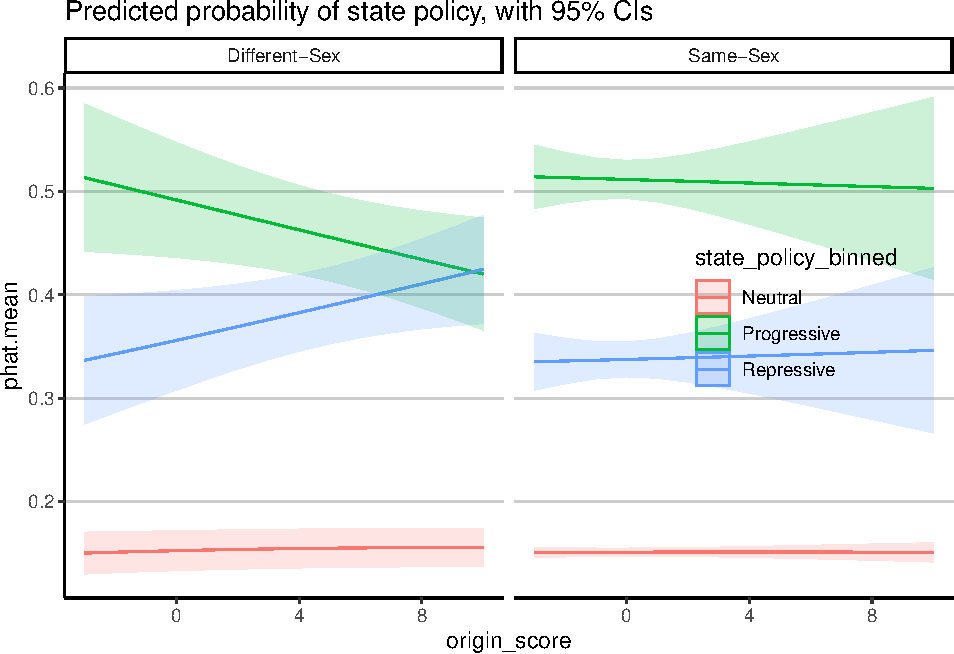
\includegraphics{ssimm_draft_methods_results_files/figure-latex/sim-1.pdf}
\caption{\label{fig:sim}Predicted probabilities of U.S. state LGBT policy progressiveness for individual immigrants in different- and same-sex couples, based on policy score of sending country, with 95\% confidence intervals.}
\end{figure}

To help interpret these results, Figure \ref{fig:sim} contains predicted probabilities of residing in progressive, neutral, or repressive U.S. states. Each panel predicts these probabilities for a typical immigrant in the dataset, based on means for continuous and modes for categorical variables while varying sending-country policy score. The only difference between the two panels is the value for the same-sex indicator.

The figure shows opposite trends for same- and different-sex couples. Overall, immigrants tend to live in more progressive states, but the moderating effect of origin score is quite different for the two groups. The panel for same-sex couples shows that these immigrants tend to live in U.S. states with similar LGBT policy contexts to those of their countries of origin. Immigrants in same-sex couples from more repressive countries are less likely to live in more progressive U.S. states, but as the origin-country score increases, so does the probability of living in a progressive state For immigrants in different-sex couples, on the other hand, increasingly progressive country-of-origin policies are associated with a \emph{lower} probability of residing in a progressive U.S. state, accompanied by a \emph{higher} probability of living in a repressive U.S. state. At the high end of the origin-score policy range, the difference in predicted probabilities is significant: typical immigrants in same-sex couples are 14 percentage points more likely to live in progressive states and -14 percentage points less likely to live in repressive states.

\hypertarget{references}{%
\section{References}\label{references}}

\setlength{\parindent}{-0.2in}
\setlength{\leftskip}{0.2in}
\setlength{\parskip}{8pt}

\noindent

\hypertarget{refs}{}
\begin{CSLReferences}{1}{0}
\leavevmode\hypertarget{ref-benson_2012}{}%
Benson, Michaela, and Karen O'Reilly. 2012. \emph{Lifestyle {Migration}: {Expectations}, {Aspirations} and {Experiences}}. Har/Ele edition. Ashgate.

\leavevmode\hypertarget{ref-fitzgerald_2018}{}%
FitzGerald, David Scott, and Rawan Arar. 2018. {``The {Sociology} of {Refugee} {Migration}.''} \emph{Annual Review of Sociology} 44 (1): 387--406. \url{https://doi.org/10.1146/annurev-soc-073117-041204}.

\leavevmode\hypertarget{ref-fitzgerald_2014}{}%
Fitzgerald, Jennifer, David Leblang, and Jessica C. Teets. 2014. {``Defying the {Law} of {Gravity}: {The} {Political} {Economy} of {International} {Migration}.''} \emph{World Politics} 66 (3): 406--45. \url{https://doi.org/10.1017/S0043887114000112}.

\leavevmode\hypertarget{ref-hatton_2005a}{}%
Hatton, Timothy J., and Jeffrey G. Williamson. 2005. \emph{Global {Migration} and the {World} {Economy}: {Two} {Centuries} of {Policy} and {Performance}}. The MIT Press. \url{https://doi.org/10.7551/mitpress/3303.001.0001}.

\leavevmode\hypertarget{ref-hernandez-leon_2013}{}%
Hernández-León, Rubén. 2013. {``Conceptualizing the Migration Industry.''} In \emph{The Migration Industry and the Commercialization of International Migration}, edited by Thomas Gammeltoft-Hansen and Ninna Nyberg Sorensen, 42--62. Routledge.

\leavevmode\hypertarget{ref-hondagneu-sotelo_2012}{}%
Hondagneu-Sotelo, Pierrette. 2012. {``New Directions in Gender and Immigration Research.''} In \emph{Routledge {International} {Handbook} of {Migration} {Studies}}. Routledge. \url{https://doi.org/10.4324/9780203863299.ch15}.

\leavevmode\hypertarget{ref-leblang_2017}{}%
Leblang, David. 2017. {``Harnessing the {Diaspora}: {Dual} {Citizenship}, {Migrant} {Return} {Remittances}.''} \emph{Comparative Political Studies} 50 (1): 75--101. \url{https://doi.org/10.1177/0010414015606736}.

\leavevmode\hypertarget{ref-lutz_2010}{}%
Lutz, Helma. 2010. {``Gender in the {Migratory} {Process}.''} \emph{Journal of Ethnic and Migration Studies} 36 (10): 1647--63. \url{https://doi.org/10.1080/1369183X.2010.489373}.

\leavevmode\hypertarget{ref-massey_1987}{}%
Massey, Douglas S., Rafael Alarcon, Jorge Durand, and Humberto González. 1987. \emph{Return to {Aztlan}: {The} {Social} {Process} of {International} {Migration} from {Western} {Mexico}}. University of California Press.

\leavevmode\hypertarget{ref-massey_1999}{}%
Massey, Douglas S., Joaquin Arango, Graeme Hugo, Ali Kouaouci, Adela Pellegrino, and J. Edward Taylor. 1999. \emph{Worlds in {Motion}: {Understanding} {International} {Migration} at the {End} of the {Millennium}}. New York: Oxford University Press.

\leavevmode\hypertarget{ref-miller_2018}{}%
Miller, Michael K., and Margaret E. Peters. 2018. {``Restraining the {Huddled} {Masses}: {Migration} {Policy} and {Autocratic} {Survival}.''} \emph{British Journal of Political Science}, March, 1--31. \url{https://doi.org/10.1017/S0007123417000680}.

\leavevmode\hypertarget{ref-piore_1979}{}%
Piore, Michael J. 1979. \emph{Birds of Passage: Migrant Labor and Industrial Societies.} Cambridge: Cambridge Univ. Press.

\leavevmode\hypertarget{ref-u.s.censusbureau_2013}{}%
U.S. Census Bureau. 2013. {``Frequently {Asked} {Questions} {About} {Same}-{Sex} {Couple} {Households}.''} U.S. Census Bureau Fertility; Family STatistics Branch.

\leavevmode\hypertarget{ref-velasco_2018}{}%
Velasco, Kristopher. 2018. {``Human {Rights} {INGOs}, {LGBT} {INGOs}, and {LGBT} {Policy} {Diffusion}, 1991--2015.''} \emph{Social Forces} 97 (1): 377--404. \url{https://doi.org/10.1093/sf/soy030}.

\leavevmode\hypertarget{ref-wallerstein_1979}{}%
Wallerstein, Immanuel. 1979. \emph{The {Capitalist} {World}-{Economy}}. Cambridge: Cambridge University Press.

\end{CSLReferences}

\end{document}
